% Number 940
% CAPMA Algebra Units 
% Softball player slide - algebraic
% JG

% Watermark
\AddToShipoutPicture*{\BackgroundPic}

\addtocounter {ProbNum} {1}

%\begin{floatingfigure}[r]{.44\textwidth}
%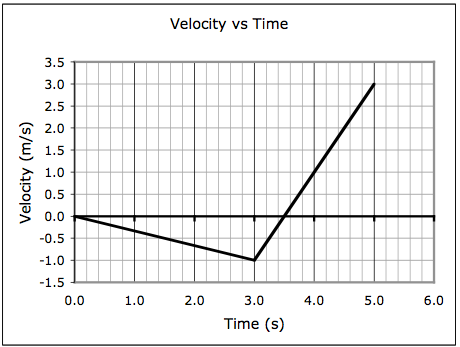
\includegraphics[scale=.54]{/Users/jgates/desktop/latex/pics/vgraph6}
%\end{floatingfigure}
 
{\bf \Large{\arabic{ProbNum}}} A softball player slides into home; as she crosses home plate, she is moving with a speed of ${3~\tfrac{m}{s}}$.  Her slide took .4 seconds and began 1.8 meters from home plate.  \bigskip

What were the magnitude (size) and direction of her acceleration during the slide? \vfill


%\begin{center}
%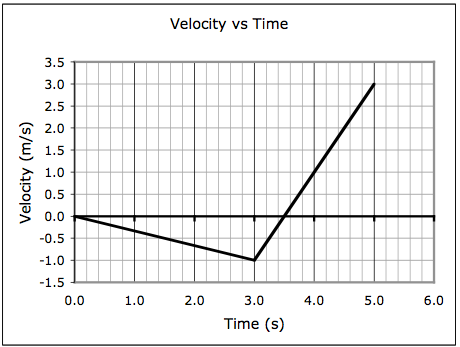
\includegraphics[scale=1]{/Users/jgates/desktop/latex/pics/vgraph6}
%\end{center}


\newpage